\section{Runtime view}
The components of the system interact with each other, in order to carry out the various activity that the system must has to accomplish.
The activity are explained from different perspective as necessary.

\subsection{Passenger makes a Request} \label{seq:passengerMakesRequest}
Components involved and their role:
\begin{itemize}
	\item \textbf{Passenger (Application)}: the activity starts when the passenger, from the mobile application, submits the request through the relative form. When the button is pressed, the client calls the method makeRequest of the Ride Handler component passing as parameters all the data of the form. He then expects as response either an affirmative message with the taxi driver info, or a negative message because there are no available taxi for the location provided.
	\item \textbf{Ride Handler}: once the Ride Handler as been called by the passenger, it firstly check whether the provided location is valid (using the Geographic Engine method) then he calls the Taxi Manager method provideTaxi, expecting a response with either a taxi or an negative message because there are no available taxi for the location provided.
	\item \textbf{Geographic Engine}: it checks if the location provided is valid or not.
	\item \textbf{Taxi Manager}: it provides a taxi for the specified location, if any available. For further details see \ref{seq:provisionOfATaxi}.
\end{itemize}
\begin{figure}[H]
	\centering
	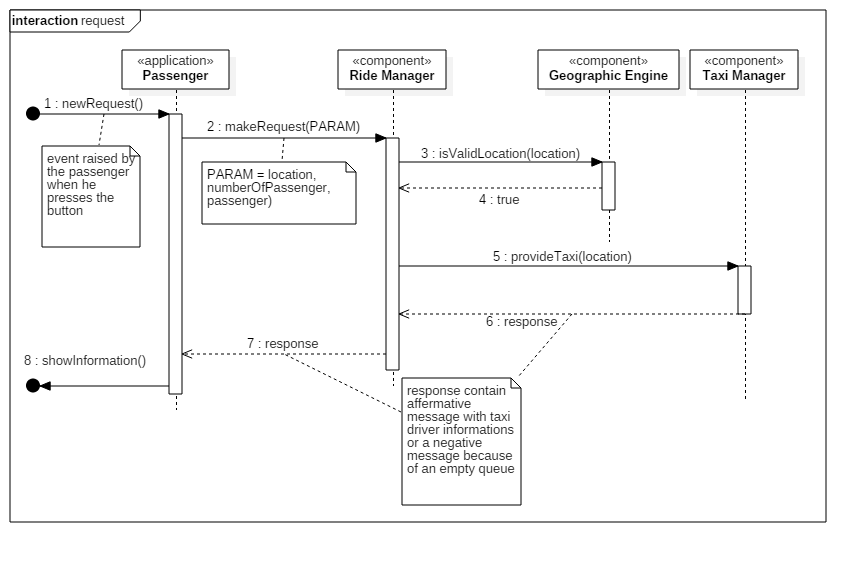
\includegraphics[scale=0.5]{../"Analysis Documents"/request}
	\label{fig:request_seq}
	\caption{Sequence Diagram of the request}
\end{figure}

\subsection{Passenger makes a Reservation}\label{seq:passengerMakesReservation}
Components involved and their role:
\begin{itemize}
	\item \textbf{Passenger (Application)}: the activity starts when the passenger, from the mobile application, submits the reservation through the relative form. When the button is pressed, the client calls the method makeReservation of the Ride Handler component passing as parameters all the data of the form. He expects as a response the outcome of the submission. Unless the location provided is not valid, the response is affirmative. The Passenger application now keeps behaving as usual and gets called by the system less then 10 minutes before the meeting time with the information of the taxi driver.
	\item \textbf{Ride Handler}: once the Ride Handler as been called by the passenger, it firstly check whether the provided location is valid (using the Geographic Engine method) then sends to the passenger the outcome of the reservation. After that, before looking for a taxi driver who will serve the reservation, he waits until 10 minutes before the meeting time. Once he wakes up, he calls the Taxi Manager method provideTaxi, expecting a response with either a taxi or an negative message because there are no available taxi for the location provided. In case the response is negative, he keeps calling the provideTaxi method until he finds an available taxi driver.
	\item \textbf{Geographic Engine}: it checks if the location provided is valid or not.
	\item \textbf{Taxi Manager}: it provides a taxi for the specified location, if any available. For further details see \ref{seq:provisionOfATaxi}.
\end{itemize}
\begin{figure}[H]
	\centering
	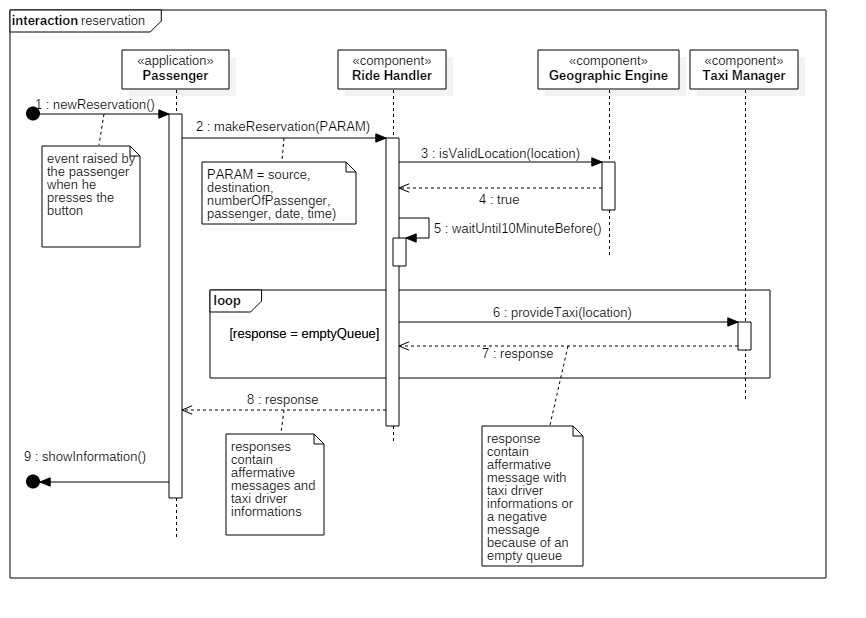
\includegraphics[scale=0.5]{../"Analysis Documents"/reservation}
	\label{fig:reservation_seq}
	\caption{Sequence Diagram of the reservation}
\end{figure}

\subsection{Provision of a taxi}\label{seq:provisionOfATaxi}
Components involved and their role:
\begin{itemize}
	\item \textbf{Taxi Manager}: it is playing the most important role of for the activity. First it gets the zone corresponding to the location from the Geographic Engine. Then he starts with a loop until either he finds a taxi driver who accepts the request, or the queue of the zone provided is empty. Every cycle it calls the method getTaxi of the Queue Manager to get a taxi driver. It then contacts the taxi driver by asking if he accepts to give a ride from a location. If the taxi driver accepts, the taxi manager returns to the caller the informations of the taxi driver. If the taxi driver does not accept, it first put them back to the queue (causing the taxi driver to be in the last position) and then it asks for a new taxi driver. Eventually, when the queue is empty, he return a negative response.
	\item \textbf{Taxi Driver (Application)}: here the taxi driver is not a single application, but it refers to the current taxi driver being called by the taxi manager. When the application receive an offer of a request, it just shows a pop up to the user and let him decide whether to accept or not the request. Then it sends the response back to the taxi manager.
	\item \textbf{Geographic Engine}: it retrieves the corresponding zone of a location
	\item \textbf{Queue Manager}: after it is called by the taxi manager, he returns the first taxi driver in the corresponding queue of the zone provided. If the queue is  empty it returns a negative response. Eventually it also put back in the queue a taxi driver who did not accept a request.
\end{itemize}
\begin{figure}[H]
	\centering
	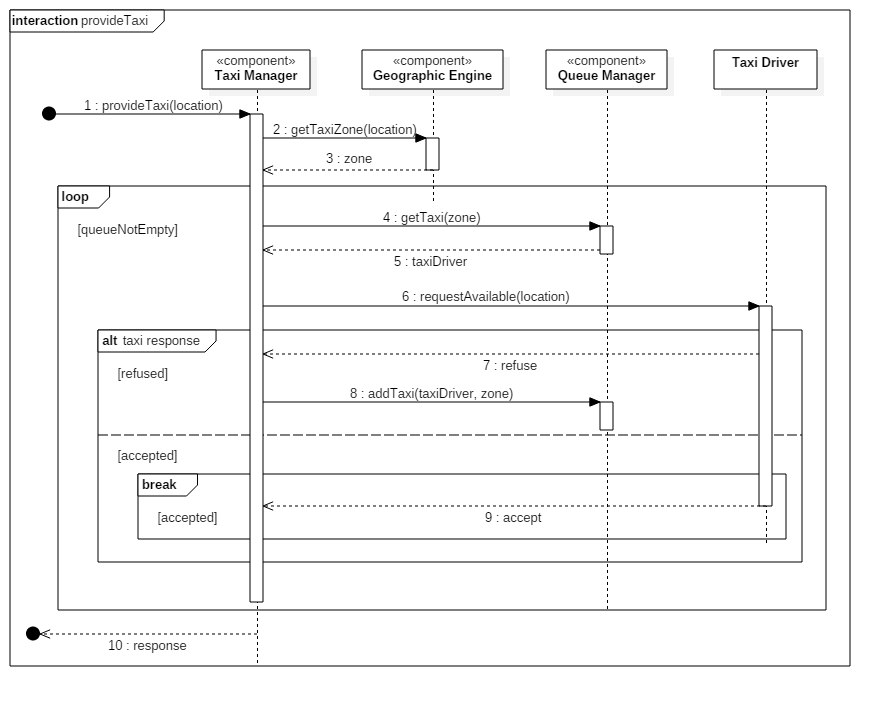
\includegraphics[scale=0.5]{../"Analysis Documents"/provideTaxi}
	\label{fig:provideTaxi_seq}
	\caption{Sequence Diagram of the provision of a taxi}
\end{figure}